\documentclass{article}
\usepackage{tikz,amsmath,tkz-graph,caption,float}
\usetikzlibrary{shapes,arrows,fit,calc,positioning,decorations.pathreplacing}
\tikzset{box/.style={draw, thick, text centered, minimum height=0.5cm, minimum width=1cm}}
\tikzset{line/.style={draw, thick, -latex'}}
\title{CSC 226 Problem Set 1 Written Part}
\author{%
	Oliver Tonnesen\\
	V00885732}
\date{September 29, 2018}
\begin{document}
\maketitle
\section{Lower bounds for sorting}
	We define $S_m$ to be the sequence $\{x_{(m-1)k+1},x_{(m-1)k+2}\ldots{x_{mk}}\}$.\\
	\newline
	\newline
	\newline
	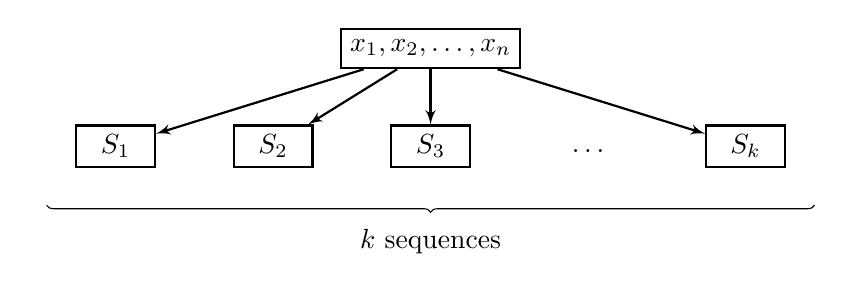
\begin{tikzpicture}
		\node [box]										(1) {${x_1,x_2,\ldots,x_n}$};
		\node [box, below=0.7cm of 1, xshift=-4cm]		(2) {$S_1$};
		\node [box, below=0.7cm of 1, xshift=-2cm]		(3) {$S_2$};
		\node [box, below=0.7cm of 1, xshift=0cm]		(4) {$S_3$};
		\node [below=0.9cm of 1, xshift=2cm]			(5) {$\ldots$};
		\node [box, below=0.7cm of 1, xshift=4cm]		(6) {$S_k$};
		\node [below=0.9cm of 1, xshift=-5cm]			(L) {};
		\node [below=0.9cm of 1, xshift=5cm]			(R) {};

		\path [line] (1) -> (2);
		\path [line] (1) -> (3);
		\path [line] (1) -> (4);
		% \path [line] (1) -> (5);
		\path [line] (1) -> (6);

		\draw [decoration={brace,mirror,raise=20pt}, decorate] (L) -- node [style={below=25pt}, pos=0.5] {$k$ sequences} (R);
	\end{tikzpicture}
	\newline
	\newline
	\newline
	Since each sequence is of length $k$, each can be sorted in $\Omega(k\log{k})$ comparisons. $k$ sequences need to be sorted,
	so sorting the entire sequence takes $\Omega(k^2\log{k})$ comparisons. Note that $k^2=n$, so $\Omega(k^2\log{k})$ is equivalent
	to ${\Omega(n\log{k})}$, and so the entire sequence can therefore be sorted in $\Omega(n\log{k})$ time.
\section{Quickselect with median-of-medians pivots}
	For each iteration of select finding the median of medians, at least half of the medians are $\ge$ the actual median of medians.
	So at least half of the $~\frac{n}{9}$ groups contribute $\ge5$ elements that are greater than the median of medians (assuming distinct elements).
	\[5\cdot\frac{1}{2}\cdot\frac{n}{9}=\frac{5n}{18}\]
	So at least $\frac{5n}{18}$ elements are greater than the median of medians. Conversely, at most $\frac{13n}{18}$ elements are lesser than the
	median of medians, and likewise at most $\frac{13n}{18}$ elements are greater than the median of medians. So we can set up our recurrence as follows:
	\[T(n)=T{\bigg(\frac{13n}{18}\bigg)}+T{\bigg(\frac{n}{9}\bigg)}+cn\]
	\begin{tikzpicture}[every node/.style={minimum size=.5cm-\pgflinewidth, outer sep=0pt}]
		\node [below=0.9cm of 1,xshift=10cm,yshift=2cm]			(top) {};
		\node [below=0.9cm of 1,xshift=10cm,yshift=-5cm]			(bottom) {};
		\draw [decoration={brace,raise=20pt}, decorate] (top) -- node [style={right=25pt}, pos=0.5] {$\infty$} (bottom);

		\filldraw[draw=black,fill=white] (0,0) rectangle (9,-1) node[pos=.5] {$cn$};
		\filldraw[draw=black,fill=white] (0,-1) rectangle (7,-2) node[pos=.5] {$\frac{7cn}{9}$};
		\filldraw[draw=black,fill=white] (7,-1) rectangle (8,-2) node[pos=.5] {$\frac{cn}{9}$};
		\filldraw[draw=black,fill=white] (0,-2) rectangle (5.44,-3) node[pos=.5] {$\frac{7cn}{9}$};
		\filldraw[draw=black,fill=white] (5.44,-2) rectangle (6.22,-3) node[pos=.5] {$\frac{7cn}{81}$};
		\filldraw[draw=black,fill=white] (6.22,-2) rectangle (7,-3) node[pos=.5] {$\frac{7cn}{81}$};
		\filldraw[draw=black,fill=white] (7,-2) rectangle (7.11,-3) node[pos=.5,yshift=-10mm] {$\frac{cn}{81}$};
		\filldraw[draw=white,fill=white] (0,-3.01) rectangle (9,-5) node[pos=.5] {\vdots};
		\filldraw[draw=black,fill=white] (3.5,-5.01) rectangle (5.5,-6) node[pos=.5] {Base Case};
	\end{tikzpicture}
	\newline
	\begin{align*}
		&=\sum_{i=0}^{\infty}cn{\bigg(\frac{15}{18}\bigg)}^i\\
		&=\frac{cn}{1-\frac{15}{18}}\\
		&=6cn\\
		&\in{O(n)}
	\end{align*}
\section{Insertion in 2\--3 trees}
\captionsetup[figure]{labelformat=empty}
	\begin{figure}[H]
		\centering
		\begin{minipage}{.33\textwidth}
			\centering
			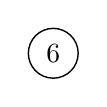
\begin{tikzpicture}
	\Vertex			{6}
\end{tikzpicture}

			\caption{Step 1}
		\end{minipage}\hfill
		\begin{minipage}{.33\textwidth}
			\centering
			\documentclass[11pt]{article}
\usepackage{fancyhdr}
\pagestyle{fancy}
\newcommand\course{MATH 423}
\newcommand\hwnumber{2}
\newcommand\duedate{October 13, 2019}

\lhead{Oliver Tonnesen\\V00885732}
\chead{\textbf{\Large Project \hwnumber}}
\rhead{\course\\\duedate}


\usepackage{cite}
\usepackage{url}


\usepackage{tikz}


\usepackage{float}
\usepackage{subcaption}


\usepackage{amsmath,amsfonts,amsthm}


\begin{document}
\section{Matchings}
\subsection{Matchings in graphs}

A matching in a graph is a set of edges such that any two share no vertex.
If every vertex in the graph is the endpoint of an edge in the matching, then the matching is called \textbf{perfect}.
If the graph is bipartite, and if for every vertex in the graph, we are given an ordering of preferences for each element in the other partite set, then a \textbf{stable matching} is a perfect matching where there do not exist elements $x$ and $y$, one from each partite set, such that $x$ prefers $y$ over the element to which it is already matched, and $y$ also prefers $x$ over the element to which it is already matched.



\subsection{Stable matchings}

The Stable Matching Problem (commonly called the Stable Marriage Problem, as it is often stated in terms of men and women selecting partners to marry) originated in part when David Gale and Lloyd Shapley wondered if they could design a self-enforcing job application process \cite{Kleinberg}.
That is, given a list of job candidates with an ordering of their preferred places of work, and a list of job openings with an ordering of their most suitable applicants, can one assign applicants to jobs in such a way that no job candidate would rather work somewhere that would also rather employ them? This question eventually lead to the Gale-Shapley algorithm.


\subsection{Applications}

Some potential applications of the Stable Matching Problem are load balancing clients to low-latency servers, and servers to clients that cost the least to serve \cite{LoadBalance}, assigning graduating medical students to hospitals, or helping transplant patients whose loved ones' organs are incompatible find suitable donors \cite{Kidney}.


\subsection{Examples}

Given two sets: $\{1,2,3\}$ and $\{A,B,C\}$ and the following preference lists:
\begin{align*}
	1: C,A,B&\qquad A: 1,2,3\\
	2: B,A,C&\qquad B: 3,2,1\\
	3: C,B,A&\qquad C: 1,3,2,
\end{align*}
a stable matching is:
\begin{figure}[H]
\centering
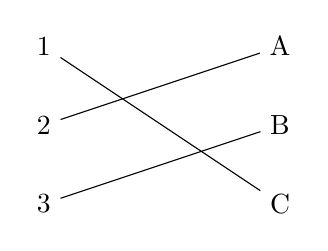
\begin{tikzpicture}[black/.style={circle,draw,fill=black,inner sep=0pt, minimum width=4pt}]
\node at (1,2) (1) {1};
\node at (1,1) (2) {2};
\node at (1,0) (3) {3};
\node at (4,2) (A) {A};
\node at (4,1) (B) {B};
\node at (4,0) (C) {C};
\draw (1) -- (C);
\draw (2) -- (A);
\draw (3) -- (B);
\end{tikzpicture}

\end{figure}


\section{Finding a stable matching}

\subsection{Gale-Shapley algorithm}

For convenience, We explain the Gale-Shapley algorithm in terms of men and women marrying.
The algorithm works by allowing women to change their mind, instead of being forced to marry the first man who proposes to her despite a more optimal partner proposing later on.
The algorithm operates as follows:

\noindent
Repeat the following until all men and women are engaged:\\ (1) Find an unpaired man $m$.
\ (2) Have $m$ propose to the woman $w$ highest on his preference list and to whom he has not already proposed.
\ (3) If $w$ prefers $m$ to her current partner (if any) then $w$ dumps her current partner, and $m$ and $w$ become engaged.


\subsection{Examples}

Given two sets: $\{m1,m2,m3,m4,m5\}$ and $\{w1,w2,w3,w4,w5\}$ and the following preference lists:
\begin{align*}
	m1: w3,w2,w5,w1,w4&\qquad w1: m3,m5,m2,m1,m4\\
	m2: w1,w2,w5,w3,w4&\qquad w2: m5,m2,m1,m4,m3\\
	m3: w4,w3,w2,w1,w5&\qquad w3: m4,m3,m5,m1,m2\\
	m4: w1,w3,w4,w2,w5&\qquad w4: m1,m2,m3,m4,m5\\
	m5: w1,w2,w4,w5,w3&\qquad w5: m2,m3,m4,m1,m5
\end{align*}

We apply the Gale-Shapley algorithm.
Between any two figures below we add as many edges as we can until we reach a conflict.
In such a conflicting scenario, a dashed line represents the new proposed partnership, green indicates that the current partnership remains, and red indicates that the standing partnership is broken in favour of the new one.

\begin{figure}[H]
\centering
\begin{subfigure}{.33\textwidth}
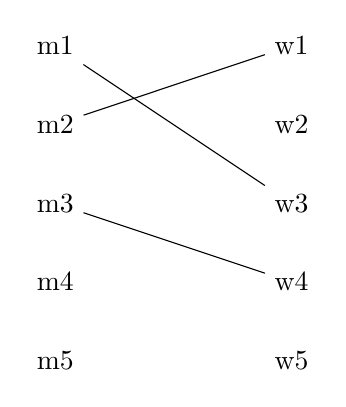
\begin{tikzpicture}[black/.style={circle,draw,fill=black,inner sep=0pt, minimum width=4pt}]
\node at (1,4) (m1) {m1};
\node at (1,3) (m2) {m2};
\node at (1,2) (m3) {m3};
\node at (1,1) (m4) {m4};
\node at (1,0) (m5) {m5};
\node at (4,4) (w1) {w1};
\node at (4,3) (w2) {w2};
\node at (4,2) (w3) {w3};
\node at (4,1) (w4) {w4};
\node at (4,0) (w5) {w5};

\draw (m1) -- (w3);
\draw (m2) -- (w1);
\draw (m3) -- (w4);
\end{tikzpicture}

\end{subfigure}
\begin{subfigure}{.33\textwidth}
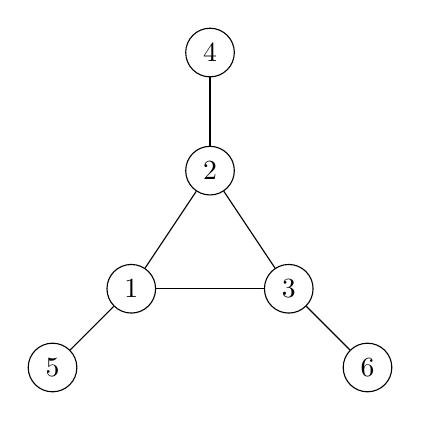
\begin{tikzpicture}[black/.style={circle,draw,fill=black,inner sep=0pt, minimum width=4pt}]
\node[circle,draw] at (1,1) (1) {1};
\node[circle,draw] at (0,0) (5) {5};
\node[circle,draw] at (3,1) (3) {3};
\node[circle,draw] at (2,2.5) (2) {2};
\node[circle,draw] at (2,4) (4) {4};
\node[circle,draw] at (4,0) (6) {6};

\draw (1) -- (2);
\draw (1) -- (3);
\draw (2) -- (3);
\draw (4) -- (2);
\draw (5) -- (1);
\draw (6) -- (3);
\end{tikzpicture}

\end{subfigure}
\end{figure}
\begin{figure}[H]
\centering
\begin{subfigure}{.33\textwidth}
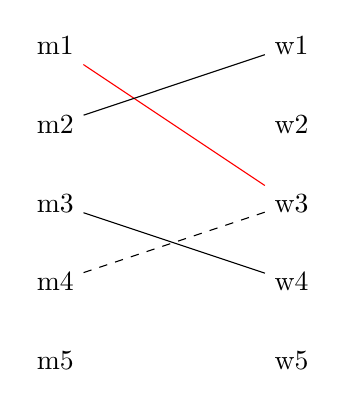
\begin{tikzpicture}[black/.style={circle,draw,fill=black,inner sep=0pt, minimum width=4pt}]
\node at (1,4) (m1) {m1};
\node at (1,3) (m2) {m2};
\node at (1,2) (m3) {m3};
\node at (1,1) (m4) {m4};
\node at (1,0) (m5) {m5};
\node at (4,4) (w1) {w1};
\node at (4,3) (w2) {w2};
\node at (4,2) (w3) {w3};
\node at (4,1) (w4) {w4};
\node at (4,0) (w5) {w5};

\draw[red] (m1) -- (w3);
\draw (m2) -- (w1);
\draw (m3) -- (w4);
\draw[dashed] (m4) -- (w3);
\end{tikzpicture}

\end{subfigure}
\begin{subfigure}{.33\textwidth}
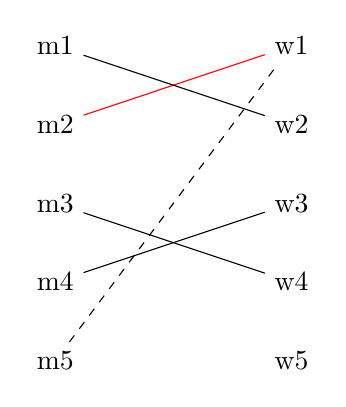
\begin{tikzpicture}[black/.style={circle,draw,fill=black,inner sep=0pt, minimum width=4pt}]
\node at (1,4) (m1) {m1};
\node at (1,3) (m2) {m2};
\node at (1,2) (m3) {m3};
\node at (1,1) (m4) {m4};
\node at (1,0) (m5) {m5};
\node at (4,4) (w1) {w1};
\node at (4,3) (w2) {w2};
\node at (4,2) (w3) {w3};
\node at (4,1) (w4) {w4};
\node at (4,0) (w5) {w5};

\draw[red] (m2) -- (w1);
\draw (m3) -- (w4);
\draw (m4) -- (w3);
\draw (m1) -- (w2);
\draw[dashed] (m5) -- (w1);
\end{tikzpicture}

\end{subfigure}
\end{figure}
\begin{figure}[H]
\centering
\begin{subfigure}{.33\textwidth}
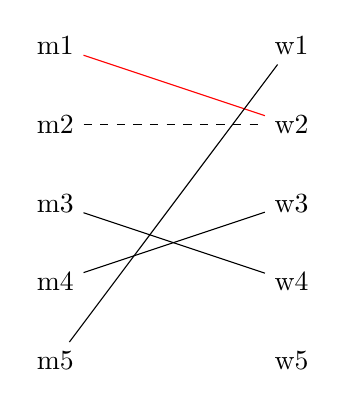
\begin{tikzpicture}[black/.style={circle,draw,fill=black,inner sep=0pt, minimum width=4pt}]
\node at (1,4) (m1) {m1};
\node at (1,3) (m2) {m2};
\node at (1,2) (m3) {m3};
\node at (1,1) (m4) {m4};
\node at (1,0) (m5) {m5};
\node at (4,4) (w1) {w1};
\node at (4,3) (w2) {w2};
\node at (4,2) (w3) {w3};
\node at (4,1) (w4) {w4};
\node at (4,0) (w5) {w5};

\draw (m3) -- (w4);
\draw (m4) -- (w3);
\draw[red] (m1) -- (w2);
\draw (m5) -- (w1);
\draw[dashed] (m2) -- (w2);
\end{tikzpicture}

\end{subfigure}
\begin{subfigure}{.33\textwidth}
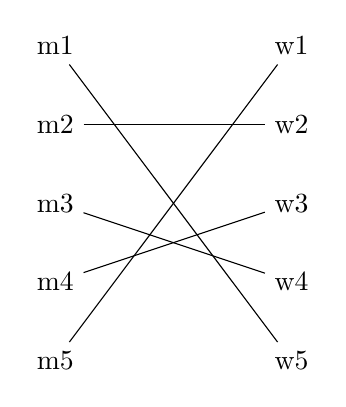
\begin{tikzpicture}[black/.style={circle,draw,fill=black,inner sep=0pt, minimum width=4pt}]
\node at (1,4) (m1) {m1};
\node at (1,3) (m2) {m2};
\node at (1,2) (m3) {m3};
\node at (1,1) (m4) {m4};
\node at (1,0) (m5) {m5};
\node at (4,4) (w1) {w1};
\node at (4,3) (w2) {w2};
\node at (4,2) (w3) {w3};
\node at (4,1) (w4) {w4};
\node at (4,0) (w5) {w5};

\draw (m3) -- (w4);
\draw (m4) -- (w3);
\draw (m5) -- (w1);
\draw (m2) -- (w2);
\draw (m1) -- (w5);
\end{tikzpicture}

\end{subfigure}
\end{figure}


\subsection{Correctness of the algorithm}

We want to show that by the end of the algorithm's execution, we're left with a stable matching.
\newline

\noindent
We first show that the algorithm produces a matching:
\newline

At any point during the execution of the algorithm, if $m$ and $w$ are matched, then $m$ was previously unmatched, and $w$ was either previously not matched, or she dumped her previous partner to be with $m$.
In either case, $m$ is matched only with $w$, and $w$ is matched only with $m$, so what we're left with is indeed a matching.
\newline

\noindent
We now show that the matching the algorithm produces is perfect:
\newline

Suppose that there exists a man $m$ who is unmatched by the end of the algorithm's execution.
Then, since there are an equal number of men and women, and since everyone is matched with at most one other person, there must exist a woman $w$ who is also unmatched.
This is not possible, since at some point, $m$ would have proposed to $w$, and $w$ would have accepted, since she was unmatched at the time.
Thus the matching produced must also be perfect.
\newline

\noindent
Finally, we show that the perfect matching produced by the algorithm is stable:
\newline

Assume that the matching the algorithm produces is not stable.
Then there exists a pair $(m,w)$ such that $m$ and $w$ are not married, but $m$ prefers $w$ over his wife, and $w$ prefers $m$ over her husband.
Let $w'$ and $m'$ be $m$'s and $w$'s spouses, respectively.
Since $w'$ is lower on $m$'s preference list than $w$, $m$ must have proposed to $w$ earlier in the algorithm's execution, but $m'$ is lower on $w$'s preference list than $m$, so $w$ would have either not accepted $m'$'s proposal, or would have dropped $m'$ in favour of $m$ at the time of $m$'s proposal.
Thus our assumption was false, and so no such pair $(m,w)$ exists, and the matching is therefore stable. \cite{Kleinberg}



\section{Further remarks}

A particularly interesting application of Gale and Shapley's algorithm, described in \cite{Kidney}, is helping transplant patients receive kidneys.
If a transplant patient has a friend or family member who is willing to give their kidney, but for some reason is incompatible with the recipient, then the Gale-Shapley algorithm can be used to find a stable matching between kidney donors and recipients such that every transplant patient receives a kidney with which they are compatible.
During the first year this program was run, it increased the rate of kidney transplants by around twenty times, and its creator, Alvin Roth, received a Nobel Prize in Economics.


% \section{References}
\bibliography{p2}
\bibliographystyle{plain}


\end{document}

			\caption{Step 2}
		\end{minipage}\hfill
		\begin{minipage}{.25\textwidth}
			\centering
			\documentclass[11pt]{article}
\usepackage{fancyhdr}
\pagestyle{fancy}
\newcommand\course{MATH 423}
\newcommand\hwnumber{3}
\newcommand\duedate{October 31, 2019}

\lhead{Oliver Tonnesen\\V00885732}
\chead{\textbf{\Large Project \hwnumber}}
\rhead{\course\\\duedate}


\usepackage{cite}
\usepackage{url}


\usepackage{tikz}
\newcount\mycount


\usepackage{float}
\usepackage{subcaption}


\usepackage{amsmath,amsfonts,amsthm}


\begin{document}
\section{Definition and characterizations}
\subsection{Definition of a line graph}
A line graph of a simple graph $G$, $L(G)$, is the graph obtained by taking
$E(G)$ to be its vertex set, and connecting two vertices with an edge if the
corresponding edges in $G$ share a common vertex.

Some definitions we use throughout this survey, assume $H$ is a suspected line
graph and $G$ is its root graph if it exists:
\newline
\underline{\textbf{$g$-clique}}: If $g\in G$, a $g$-clique in $H$ is a clique
in $H$, corresponding to the star graph centred at $g$ in $G$.
\newline
\underline{\textbf{Half-named}}: A vertex in $H$ is "half-named" when it
corresponds to an edge of $G$, one of whose vertices belongs to a fully
discovered $g$-clique in $H$.
\newline
\underline{\textbf{Fully named}}: A vertex in $H$ is "fully named" when it
corresponds to an edge of $G$, both of whose vertices belong to a fully
discovered $g$-clique in $H$.
\newline
\underline{\textbf{Even triangle}}: A triangle such that every vertex in the
graph is adjacent to exactly two or zero vertices in the triangle.
\newline
\underline{\textbf{Odd triangle}}: A triangle  such that every vertex in the
graph is adjacent to exactly one or three vertices in the triangle.
\newline
\underline{\textbf{Cross vertex}}: Given two vertices in $H$ $x-y$ and $y-z$,
a cross vertex is one of the form the name $x-z$.


\subsection{Examples}
\begin{figure}[H]
\centering
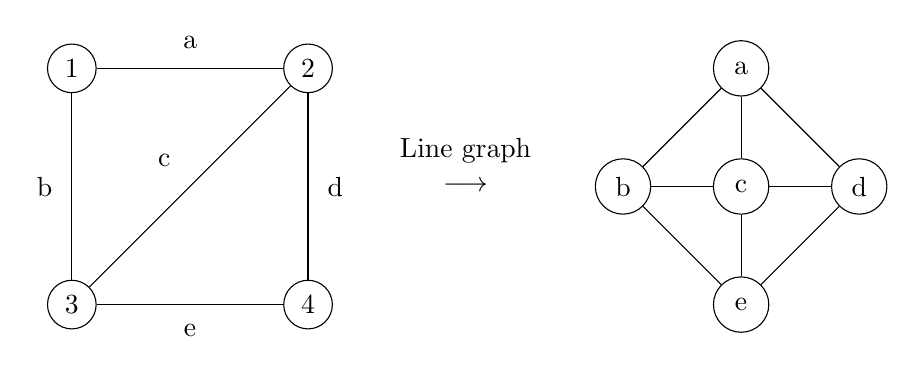
\begin{tikzpicture}[black/.style={circle,draw,fill=black,inner sep=0pt, minimum width=4pt}]
\node[circle,draw] at (0,3) (1) {1};
\node[circle,draw] at (3,3) (2) {2};
\node[circle,draw] at (0,0) (3) {3};
\node[circle,draw] at (3,0) (4) {4};

\draw (1) -- (2) node [midway,label=above:{a}] {};
\draw (1) -- (3) node [midway,label=left:{b}] {};
\draw (2) -- (3) node [midway,label=above left:{c}] {};
\draw (2) -- (4) node [midway,label=right:{d}] {};
\draw (3) -- (4) node [midway,label=below:{e}] {};


\draw node at (5, 1.5) {$\longrightarrow$};
\draw[above,yshift=5] node at (5,1.5) {Line graph};


\node[circle,draw,minimum width=20pt] at (8.5,3) (a) {a};
\node[circle,draw,minimum width=20pt] at (7,1.5) (b) {b};
\node[circle,draw,minimum width=20pt] at (8.5,1.5) (c) {c};
\node[circle,draw,minimum width=20pt] at (10,1.5) (d) {d};
\node[circle,draw,minimum width=20pt] at (8.5,0) (e) {e};

\draw (a) -- (b);
\draw (a) -- (c);
\draw (a) -- (d);
\draw (b) -- (c);
\draw (b) -- (e);
\draw (c) -- (d);
\draw (c) -- (e);
\draw (d) -- (e);
\end{tikzpicture}

\end{figure}
\begin{figure}[H]
\centering
\begin{tikzpicture}[black/.style={circle,draw,fill=black,inner sep=0pt,minimum width=4pt}]
\node[black] at (0,0) (0) {};
\foreach \number in {1,...,8}
{
	\mycount=\number
	\advance\mycount by -1
	\multiply\mycount by 45
	\advance\mycount by 0
	\node[black] (\number) at (\the\mycount:1cm) {};
	\draw (0) -- (\number);
}


\draw node at (3, 0) {$\longrightarrow$};
\draw[above,yshift=5] node at (3,0) {Line graph};


\foreach \number in {1,...,8}
{
	\mycount=\number
	\advance\mycount by -1
	\multiply\mycount by 45
	\advance\mycount by 0
	\node[black,xshift=160] (\number) at (\the\mycount:1cm) {};
}
\foreach \x in {1,...,8}
	\foreach \y in {\x,...,8}
		\draw (\x) -- (\y);


\end{tikzpicture}

\end{figure}


\subsection{Characterizations of line graphs by forbidden structures and by forbidden subgraphs}
A graph is the line graph of some simple graph if and only if it contains none
of these nine graphs as induced subgraphs\cite{vanRooij}:

\begin{figure}[H]
\centering
	\begin{minipage}{.3\textwidth}
		\centering
		\begin{tikzpicture}[black/.style={circle,draw,fill=black,inner sep=0pt, minimum width=4pt}]
\node[black] at (0,0) (0) {};
\foreach \number in {1,...,3}
{
	\mycount=\number
	\advance\mycount by -1
	\multiply\mycount by 120
	\advance\mycount by 0
	\node[black] (\number) at (\the\mycount:1cm) {};
	\draw (0) -- (\number);
}
\end{tikzpicture}

	\end{minipage}
	\begin{minipage}{.3\textwidth}
		\centering
		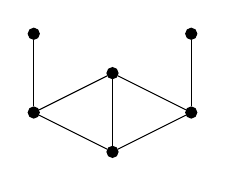
\begin{tikzpicture}[black/.style={circle,draw,fill=black,inner sep=0pt, minimum width=4pt}]
\node[black] at (1,0)	(0) {};
\node[black] at (0,0.5)	(1) {};
\node[black] at (2,0.5)	(2) {};
\node[black] at (1,1)	(3) {};
\node[black] at (0,1.5)	(4) {};
\node[black] at (2,1.5)	(5) {};

\draw (0) -- (1);
\draw (0) -- (2);
\draw (0) -- (3);
\draw (3) -- (1);
\draw (3) -- (2);
\draw (4) -- (1);
\draw (5) -- (2);
\end{tikzpicture}

	\end{minipage}
	\begin{minipage}{.3\textwidth}
		\centering
		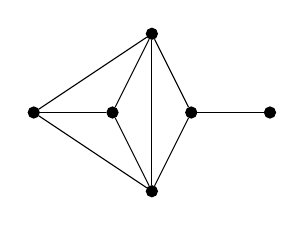
\begin{tikzpicture}[black/.style={circle,draw,fill=black,inner sep=0pt, minimum width=4pt}]
\node[black] at (0,0)	(0) {};
\node[black] at (1,0)	(1) {};
\node[black] at (1.5,1)	(2) {};
\node[black] at (1.5,-1)(3) {};
\node[black] at (2,0)	(4) {};
\node[black] at (3,0)	(5) {};

\draw (0) -- (1);
\draw (0) -- (2);
\draw (0) -- (3);
\draw (1) -- (2);
\draw (1) -- (3);
\draw (2) -- (3);
\draw (4) -- (2);
\draw (4) -- (3);
\draw (4) -- (5);
\end{tikzpicture}

	\end{minipage}
\end{figure}
\begin{figure}[H]
\centering
	\begin{minipage}{.3\textwidth}
		\centering
		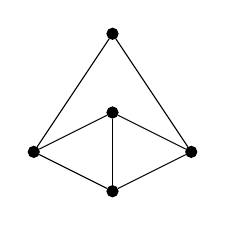
\begin{tikzpicture}[black/.style={circle,draw,fill=black,inner sep=0pt, minimum width=4pt}]
\node[black] at (1,0)	(0) {};
\node[black] at (0,0.5)	(1) {};
\node[black] at (2,0.5)	(2) {};
\node[black] at (1,1)	(3) {};
\node[black] at (1,2)	(4) {};

\draw (0) -- (1);
\draw (0) -- (2);
\draw (0) -- (3);
\draw (1) -- (3);
\draw (2) -- (3);
\draw (4) -- (1);
\draw (4) -- (2);
\end{tikzpicture}

	\end{minipage}
	\begin{minipage}{.3\textwidth}
		\centering
		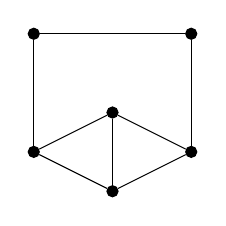
\begin{tikzpicture}[black/.style={circle,draw,fill=black,inner sep=0pt, minimum width=4pt}]
\node[black] at (1,0)	(0) {};
\node[black] at (0,0.5)	(1) {};
\node[black] at (2,0.5)	(2) {};
\node[black] at (1,1)	(3) {};
\node[black] at (0,2)	(4) {};
\node[black] at (2,2)	(5) {};

\draw (0) -- (1);
\draw (0) -- (2);
\draw (0) -- (3);
\draw (1) -- (3);
\draw (2) -- (3);
\draw (4) -- (1);
\draw (5) -- (2);
\draw (5) -- (4);
\end{tikzpicture}

	\end{minipage}
	\begin{minipage}{.3\textwidth}
		\centering
		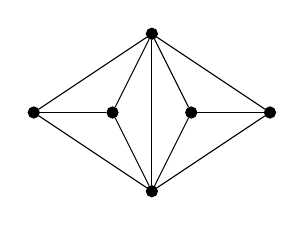
\begin{tikzpicture}[black/.style={circle,draw,fill=black,inner sep=0pt, minimum width=4pt}]
\node[black] at (0,0)	(0) {};
\node[black] at (1,0)	(1) {};
\node[black] at (1.5,1)	(2) {};
\node[black] at (1.5,-1)(3) {};
\node[black] at (2,0)	(4) {};
\node[black] at (3,0)	(5) {};

\draw (0) -- (1);
\draw (0) -- (2);
\draw (0) -- (3);
\draw (1) -- (2);
\draw (1) -- (3);
\draw (2) -- (3);
\draw (4) -- (2);
\draw (4) -- (3);
\draw (4) -- (5);
\draw (5) -- (2);
\draw (5) -- (3);
\end{tikzpicture}

	\end{minipage}
\end{figure}
\begin{figure}[H]
\centering
	\begin{minipage}{.3\textwidth}
		\centering
		\begin{tikzpicture}[black/.style={circle,draw,fill=black,inner sep=0pt, minimum width=4pt}]
\node[black] at (0,0) (0) {};
\foreach \x in {1,...,5}
{
	\mycount=\x
	\advance\mycount by -1
	\multiply\mycount by 72
	\advance\mycount by 18
	\node[black] (\x) at (\the\mycount:1cm) {};
	\draw (0) -- (\x);
}
\foreach \x in {1,...,4}
{
	\mycount=\x
	\advance\mycount by 1
	\draw (\x) -- (\the\mycount);
}
\draw (1) -- (5);
\end{tikzpicture}

	\end{minipage}
	\begin{minipage}{.3\textwidth}
		\centering
		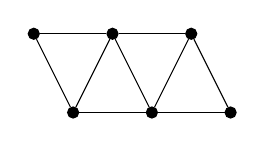
\begin{tikzpicture}[black/.style={circle,draw,fill=black,inner sep=0pt, minimum width=4pt}]
\foreach \x in {0,...,2}
{
	\node[black] at (\x, 1) (a\x) {};
	\node[black] at (\x+0.5, 0) (b\x) {};
	\draw (a\x) -- (b\x);
}
\foreach \x/\y in {0/1,1/2}
{
	\draw (a\x) -- (a\y);
	\draw (b\x) -- (b\y);
	\draw (b\x) -- (a\y);
}
\end{tikzpicture}

	\end{minipage}
	\begin{minipage}{.3\textwidth}
		\centering
		\begin{tikzpicture}[black/.style={circle,draw,fill=black,inner sep=0pt, minimum width=4pt}]
\node[black] at (0,0) (0) {};
\foreach \x in {1,...,4}
{
	\mycount=\x
	\advance\mycount by -1
	\multiply\mycount by 90
	\advance\mycount by 0
	\node[black] (\x) at (\the\mycount:1cm) {};
	\draw (0) -- (\x);
}
\foreach \x in {1,...,3}
{
	\mycount=\x
	\advance\mycount by 1
	\draw (\x) -- (\the\mycount);
}
\draw (1) -- (4);
\draw (2) to[out=0,in=90] (1.5,0) to[out=-90,in=0]  (4);
\end{tikzpicture}

	\end{minipage}
\end{figure}

Another characterization \cite{vanRooij}: A graph is a line graph of some
simple graph if and ly if it is claw-free and no induced diamond subgraph of
$G$ has two odd triangles.


\section{Recognitions}
\subsection{Lehot algorithm for constructing the root graph of a graph if it exists}
We're given a graph $G=(V(G),E(G)$. The algorithm described in \cite{Lehot} has 9 steps:
\newline
\newline
\noindent
\underline{Step 1}:
Select two adjacent vertices in $V(G)$, and name them $1-2$ and $2-3$. Call
these vertices the "basic vertices."
\newline
\newline
\noindent
\underline{Step 2}:
Find all vertices adjacent to both basic vertices. If there are at least three
such vertices, go to step 5. If ther are none, go to step 6. If there is one,
continue to step 3. If there are two, go to step 4.
\newline
\newline
\noindent
\underline{Step 3}:
Call the one vertex $x$. If the triangle $(x,1-2,2-3)$ is odd, call $x$ $2-4$
and go to step 6. Otherwise call $x$ $1-3$ and go to step 7.
\newline
\newline
\noindent
\underline{Step 4}:
Call the two vertices $x$ and $y$. If $x~y$, then $(x,1-2,2-3)$ and
$(y,1-2,2-3)$ are two distinct triangles. If one triangle, say $(x,1-2,2-3)$
is odd, then call $x$ $2-4$, call $y$ $1-3$ (note that this makes it a cross
vertex) dnd go to step 6. Otherwise both triangles are even, and the only
three possibilities are the following:
\newline
\newline
\noindent
\underline{Step 5}:
There are at least three vertices adjacent to both basic vertices. Find two
that are nonadjacent, $a$ and $b$. We check if $a$ is adjacent to a third
vertex in this set. If it is, then we call $b$ the cross vertex. If not, then
we call $a$ the cross vertex. If there are no such $a$ and $b$, continue to
step 6, otherwise go to step 7.
\newline
\newline
\noindent
\underline{Step 6}:
All the vertices in the $g$-clique are named, and we use them to half-name all
the vertices adjacent to them, then go to step 8.
\newline
\newline
\noindent
\underline{Step 7}:
All the vertices in the $g$-clique are named, and the cross vertex is fully
named.  We use the vertices of the $g$-clique to half-name the vertices
adjacent to them, then go to step 8.
\newline
\newline
\noindent
\underline{Step 8}:
If there remain no more vertices that are not fully named, continue to step 9.
Otherwise choose any half-named vertex. By definition, it is adjacent to a
fully-named vertex. If this vertex does not belong to an already discovered
$g$-clique, then there must be a fully-named vertex which \underline{does}
belong to an already discovered clique, and which is defined as the cross
vertex of the two vertices. These two vertices fully name the
previously-chosen half-named vertex. Use the vertices of this clique to
half-name all the adjacent vertices with the number in their name which is
\underline{not} the clique number ($g$), then go back to step 8.
\newline
\newline
\noindent
\underline{Step 9}:
Compare $L(G)$ to $H$. If they are isomorphic, then $H$ is a line graph, otherwise it is not.


\subsection{Apply Lehot algorithm to construct the root graph of the graph below}
\begin{figure}[H]
\centering
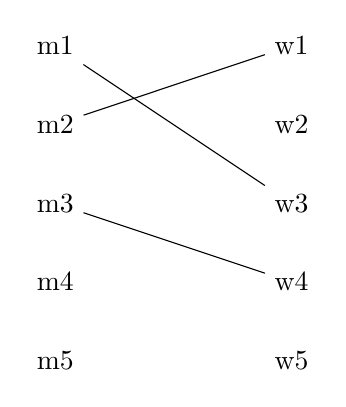
\begin{tikzpicture}[black/.style={circle,draw,fill=black,inner sep=0pt, minimum width=4pt}]
\node at (1,4) (m1) {m1};
\node at (1,3) (m2) {m2};
\node at (1,2) (m3) {m3};
\node at (1,1) (m4) {m4};
\node at (1,0) (m5) {m5};
\node at (4,4) (w1) {w1};
\node at (4,3) (w2) {w2};
\node at (4,2) (w3) {w3};
\node at (4,1) (w4) {w4};
\node at (4,0) (w5) {w5};

\draw (m1) -- (w3);
\draw (m2) -- (w1);
\draw (m3) -- (w4);
\end{tikzpicture}

\end{figure}
Starting at step 1 of the algorithm, we choose $x$ and $y$ as our basic
vertices, and name $x=1-2$ and $y=2-3$. Continuing to step 2, we find two
vertices adjacent to both basic vertices: $z$ and $v$. There are two such
verties, so we continue to step 4. $z$ and $v$ are not adjacent, so they make
two distinct triangles. The triangle $(x,y,z)$ is odd, so we call $z=2-4$, and
$v=1-3$. We now skip to step 6, and use our fully named $1-clique$ to
successively half-name all vertices adjacent to it: $w=3-6$, and $u=1-5$. Now
at step 8, we choose a half-named vertex, $u$. It is adjacent to a fully named
vertex, $x$. $x$ and $v$ fully name $u$. We continue this for the remaining
vertices, and we obtain the graph below:

\begin{figure}[H]
\centering
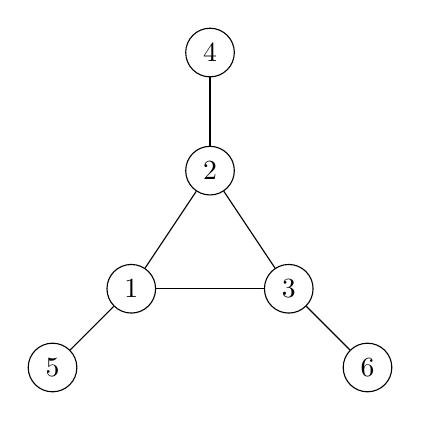
\begin{tikzpicture}[black/.style={circle,draw,fill=black,inner sep=0pt, minimum width=4pt}]
\node[circle,draw] at (1,1) (1) {1};
\node[circle,draw] at (0,0) (5) {5};
\node[circle,draw] at (3,1) (3) {3};
\node[circle,draw] at (2,2.5) (2) {2};
\node[circle,draw] at (2,4) (4) {4};
\node[circle,draw] at (4,0) (6) {6};

\draw (1) -- (2);
\draw (1) -- (3);
\draw (2) -- (3);
\draw (4) -- (2);
\draw (5) -- (1);
\draw (6) -- (3);
\end{tikzpicture}

\end{figure}

It is simple to check that the line graph of the graph below is isomorphic to
the original graph, and so the graph we were given was indeed a line graph,
and the graph we constructed is its root graph.


\section{Optimization}
\subsection{Find a maximum clique in a line graph}
Given a graph $L(G)$, finding a vertex of degree $\Delta(G)\neq3$ in $G$
corresponds to finding a maximum matching in $L(G)$. Since this algorithm runs
in linear time, if $L(G)$ is indeed the line graph of some simple graph $G$,
then we can find a maximum clique -- normally a very computationally hard
problem -- efficiently by transforming one from a degree $\Delta(G)$ vertex in
$G$.


\subsection{Find a maximum independent set in a line graph}
Given a graph $L(G)$, finding a maximum matching in $G$ corresponds to finding
a maximum independent set in $L(G)$. Since this algorithm runs in linear time,
if $L(G)$ is indeed the line graph of some simple graph $G$, then we can find
a maximum independent set -- normally a very computationally hard problem --
efficiently by transforming one from a maximum matching in $G$.


\bibliography{p3}
\bibliographystyle{plain}


\end{document}

			\caption{Step 3}
		\end{minipage}\hfill
	\end{figure}
	\begin{figure}[H]
		\centering
		\begin{minipage}{.33\textwidth}
			\centering
			\documentclass[11pt]{article}
\usepackage{fancyhdr}
\pagestyle{fancy}
\newcommand\course{MATH 423}
\newcommand\hwnumber{4}
\newcommand\duedate{November 21, 2019}

\lhead{Oliver Tonnesen\\V00885732}
\chead{\textbf{\Large Project \hwnumber}}
\rhead{\course\\\duedate}


\usepackage{cite}
\usepackage{url}


\usepackage{tikz}
\newcount\mycount


\usepackage{float}
\usepackage{subcaption}


\usepackage{amsmath,amsfonts,amsthm}


\begin{document}
\section{Introduction}
\subsection{Background}
An interval graph is a graph related to a set of intervals on the real line.
The interval graph problem was first posed by Gy\"orgy Haj\'os in 1957.
\cite{Golumbic} The problem is to determine whether or not a given graph is
isomorphic to an interval graph.


\subsection{Applications}
Interval graphs can be applied very naturally to many types of scheduling and
resource allocation problems:

If each interval represents a task to be completed, and certain tasks (namely
those with intersecting intervals) cannot be done at the same time, then
finding an independent set in the corresponding interval graph is equivalent
to finding a set of tasks that can be completed simultaneously.

If each interval represents a course needing a classroom at a particular time,
then finding an optimal colouring of the corresponding interval graph
represents an allocation of the fewest possible classrooms such that no two
courses use the same classroom at the same time.

When compiling a computer program to machine code, the compiler must store a
number of variables' values in a small number of registers. If two variables
are never used simultaneously, then they can be allocated to the same
register.  The compiler can check when the first and last use of each variable
occurs, and use these intervals to create an interval graph. The minimum
number of registers required to run the program is equal to the chromatic
number of the this interval graph.


\subsection{Definitions}
\underline{Interval Graph}: Given a family of intervals
$\{S_i\}_{i=1,\ldots,n}$, the corresponding interval graph is defined by
assigning a vertex $v_i$ to each $S_i$, and joining $v_i$ and $v_j$ with an
edge whenever $S_i\cap S_j\neq\emptyset$.

\noindent
\underline{Comparability Graph}: A comparability graph is an undirected graph
connecting pairs of elements that are comparable in a partial order.

\noindent
\underline{Clique Matrix}: Given a graph $G$, its clique matrix $M$ has rows
representing maximal cliques in $G$, and columns representing vertices in
$V(G)$, where $M_{ij}=1$ if vertex $j$ is in clique $i$, and 0 otherwise.


\section{Characterizations}
\subsection{Vertex ordering}
A graph with maximal cliques $M_1,\ldots,M_k$ is an interval graph if and only
if its cliques can be ordered in such a way that for any vertex $v$, the
maximal cliques containing $v$ occur consecutively. \cite{Golumbic}


\subsection{Forbidden subgraphs/structures}
A graph is an interval graph if and only if every induced cycle has exactly
three vertices, and its complement is a comparability graph. \cite{West}


\subsection{Clique covering}
A graph is an interval graph if and only if the rows of its clique matrix can
be permuted such that the 1s in each column appear consecutively. \cite{Fulkerson}


\section{Recognition algorithms}
Booth and Lueker\cite{Booth} showed in 1976 that given a finite set $X$ and a
collection $\mathcal{F}$ of subsets of $X$, the question of whether or not
there exists a permutation of $X$ in which the elements of each subset in
$\mathcal{F}$ appear consecutively as a subsequence of the permutation can be
decided in linear time. This can be applied to the interval graph problem as
follows:

Given a graph $G$, let $X$ be the set of maximal cliques of $G$, and let
$\mathcal{F}=\{C_v\mid v\in V(G)\}$, where $C_v$ is a maximal clique
containing $v$. If there does exist a permutation of $X$ as described above,
then by the first characterization of interval graphs we gave, $G$ is an
interval graph, and similarly if no such permutation exists, then $G$ is not
an interval graph.


\section{Optimization problems}
\subsection{Colouring}
It's clear to see that the minimum number of colours needed to properly colour
an interval graph is the same as the largest set of pairwise intersecting
intervals. In fact, if we order the vertices of an interval graph according to
the left endpoint of their interval, then a greedy colour will colour the
graph optimally. Importantly, this procedure allows an interval graph to be
coloured in linear time, whereas this problem is extremely difficult in a
general graph. \cite{Olariu}


\subsection{Maximum clique}
Every maximum clique in an interval graph is a maximum set of pairwise
intersecting intervals. As we mentioned above, the largest set of pairwise
intersecting intervals has the same size as the number of colours required to
properly colour the interval graph. So the obvious way to find a maximum
clique in an interval graph is to greedily colour it using the above given
ordering, and to take a subsequence $v_1,\ldots,v_\chi$ of the ordering such
that $v_1$ is coloured 1, and $v_{i+1}$ is the first vertex after $v_i$ to be
coloured $i+1$. $v_{i+1}$ must be adjacent to all previous vertices in the
subsequence, as if it weren't adjacent to one of them, say $v_k$, $k<i+1$, the
greedy algorithm would have coloured $v_{i+1}$ with the colour $k$ instead. So
our sequence does indeed form a clique, and that clique has size $\chi$.


\subsection{Maximum independent set}
Our second characterization of interval graphs mentioned that any induced
cycle has exactly three vertices. Graphs of this kind are also called
\underline{chordal graphs}. In 1972, Gavril presented a linear time algorithm
for finding a maximum independent set in a chordal graph. \cite{Gavril}


\subsection{Minimum clique covering}
A minimum clique covering of any graph must have at least as many vertices as
a maximum independent set. Since we're considering an interval graph, our
maximum independent set must intersect all other vertices. The existence of a
vertex not in the independent set and not intersecting the intervals of any
vertices in our independent set would violate the maximality of our
independent set. Similarly, the existence of two nonintersecting intervals
both lying inside the interval of a vertex in our independent set would also
violate the maximality of our independent set. So each vertex uniquely covers
one of each of the maximal cliques in our graph, and thus determines a clique
covering. So any minimum clique covering must have at most as many cliques as
there are vertices in our independent set. Thus in an interval graph, the
minimum clique covering contains exactly as many cliques as the number of
vertices in a maximum independent set.


\bibliography{p4}
\bibliographystyle{plain}


\end{document}

			\caption{Step 4}
		\end{minipage}\hfill
		\begin{minipage}{.33\textwidth}
			\centering
			\documentclass[11pt]{article}
\usepackage{fancyhdr}
\pagestyle{fancy}
\newcommand\course{MATH 423}
\newcommand\hwnumber{5}
\newcommand\duedate{December 2, 2019}

\lhead{Oliver Tonnesen\\V00885732}
\chead{\textbf{\Large Project \hwnumber}}
\rhead{\course\\\duedate}


\usepackage{cite}
\usepackage{url}


\usepackage{tikz}
\newcount\mycount


\usepackage{float}
\usepackage{subcaption}


\usepackage{amsmath,amsfonts,amsthm}


\begin{document}
\section{Introduction}

\subsection{Definition of split graphs}

A split graph is one that can be partitioned into a clique and an independent set.


\subsection{Examples}

$K_n\lor\overline{K_m}$:
\newline
\newline
\begin{tikzpicture}[black/.style={circle,draw,fill=black,inner sep=0pt,minimum width=4pt}]
\def\n{3}
\def\m{3}
\def\ang{90}
\foreach \number in {1,...,\n}
{
	\mycount=\number
	\advance\mycount by -1
	\multiply\mycount by \ang
	\advance\mycount by 270
	\node[black,xshift=70,yshift=57] (k\number) at (\the\mycount:1cm) {};
}
\foreach \x in {1,...,\n}
	\foreach \y in {\x,...,\n}
		\draw (k\x) -- (k\y);

\foreach \number in {1,...,\m}
{
	\node[black] (\number) at (0,\number) {};
	\foreach \x in {1,...,\n}
		\draw (\number) -- (k\x);
}
\end{tikzpicture}
\newline
\newline
$K_2$:
\newline
\newline
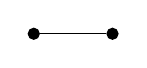
\begin{tikzpicture}[black/.style={circle,draw,fill=black,inner sep=0pt,minimum width=4pt}]
	\node[black] (a) at (0,0) {};
	\node[black] (b) at (1,0) {};
	\draw (a) -- (b);
\end{tikzpicture}
\newline
\newline
$P_4$:
\newline
\newline
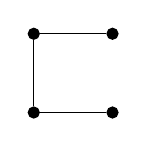
\begin{tikzpicture}[black/.style={circle,draw,fill=black,inner sep=0pt,minimum width=4pt}]
	\node[black] (a) at (0,0) {};
	\node[black] (b) at (0,1) {};
	\node[black] (c) at (1,0) {};
	\node[black] (d) at (1,1) {};
	\draw (a) -- (b);
	\draw (a) -- (c);
	\draw (b) -- (d);
\end{tikzpicture}
\newline
\newline
$K_{1,n}$:
\newline
\newline
\begin{tikzpicture}[black/.style={circle,draw,fill=black,inner sep=0pt,minimum width=4pt}]
\def\n{1}
\def\m{5}
\def\ang{90}
\foreach \number in {1,...,\n}
{
	\mycount=\number
	\advance\mycount by -1
	\multiply\mycount by \ang
	\advance\mycount by 270
	\node[black,xshift=70,yshift=114] (k\number) at (\the\mycount:1cm) {};
}
\foreach \x in {1,...,\n}
	\foreach \y in {\x,...,\n}
		\draw (k\x) -- (k\y);

\foreach \number in {1,...,\m}
{
	\node[black] (\number) at (0,\number) {};
	\foreach \x in {1,...,\n}
		\draw (\number) -- (k\x);
}
\end{tikzpicture}


\subsection{Basic properties}

\begin{itemize}
	\item If $G$ is a split graph, then $\overline{G}$ is a split graph.
	\item If $G$ is a split graph with partition $(S,K)$, $S$ an independent set and $K$
		a clique, then exactly one of the following holds:
		\begin{enumerate}
			\item $|S|=\alpha(G)$ and $|K|=\omega(G)$.
			\item $|S|=\alpha(G)$ and $|K|=\omega(G)-1$, and there exists a vertex
				$x\in S$ such that $K+x$ is a complete graph.
			\item $|S|=\alpha(G)-1$ and $|K|=\omega(G)$, and there exists a vertex
				$y\in K$ such that $S+y$ is independent.
		\end{enumerate}
	\item $G$ is a split graph if and only if both $G$ and $\overline{G}$ are chordal. \cite{Golumbic}
\end{itemize}


\section{Characterizations}

\subsection{Vertex ordering}

Let $G$ be a graph with degree sequence $d_1\le\cdots\le d_n$, and let $m$ be the largest $i$ with $d_i\ge i-1$.
Then $G$ is a split graph if and only if \[\sum_{i=1}^md_i=m(m-1)+\sum_{i=m+1}^nd_i.\]
Furthermore, if the above equality holds, then $\omega(G)=m$. \cite{Hammer}


\subsection{Forbidden subgraphs}

$G$ is a split graph if and only if $G$ contains no induced subgraph isomorphic to any of $C_4$, $\overline{C_4}$, or $C_5$. \cite{Hammer}


\section{Optimization problems}

\subsection{Colouring}

Split graphs are in particular chordal graphs.
\cite{Golumbic} gives an algorithm to colour chordal graphs in linear time, so split graphs can also be coloured in linear time.
This is a very hard problem in general, and colouring an arbitrary graph takes exponential time.


\subsection{Maximum clique}

$m$ as defined in the vertex ordering characterization of split graphs allows us to find a maximum clique: the $m$ vertices of largest degree form a maximum clique on $G$.
This process can be done in linear time.


\subsection{Maximum independent set}

Let $K$ be the maximum clique obtained using the above method.
$V(G)\setminus K$ is an independent set, so we know from the basic properties that exactly one of the three cases is possible, and $\alpha(G)$ is either $|V(G)\setminus K|$ or $|V(G)\setminus K|+1$.
If it is $|V(G)\setminus K|+1$, then there exists a vertex $y\in K$ such that $V(G)\setminus K + y$ is still independent.
We can search $K$ for such a vertex in linear time, and we're done.


\subsection{Minimum clique covering}

We know that $\overline{G}$ is a split graph, so we can colour $\overline{G}$ using the algorithm given in \cite{Golumbic} to get a set of colour classes, all of which are independent sets in $\overline{G}$, hence cliques in $G$.
Since the colouring is optimal, the corresponding clique cover is minimal.


\bibliography{p5}
\bibliographystyle{plain}


\end{document}

			\caption{Step 5}
		\end{minipage}\hfill
		\begin{minipage}{.33\textwidth}
			\centering
			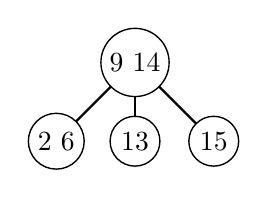
\begin{tikzpicture}
	\Vertex				{9 14}
	\Vertex[x=-1,y=-1]	{2 6}
	\Vertex[x=0,y=-1]	{13}
	\Vertex[x=1,y=-1]	{15}
	
	\Edge				(9 14)(2 6)
	\Edge				(9 14)(13)
	\Edge				(9 14)(15)
\end{tikzpicture}

			\caption{Step 6}
		\end{minipage}\hfill
	\end{figure}
	\begin{figure}[H]
		\centering
		\begin{minipage}{.33\textwidth}
			\centering
			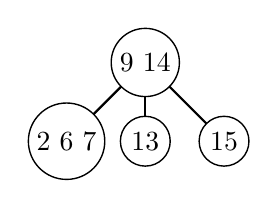
\begin{tikzpicture}
	\Vertex				{9 14}
	\Vertex[x=-1,y=-1]	{2 6 7}
	\Vertex[x=0,y=-1]	{13}
	\Vertex[x=1,y=-1]	{15}
	
	\Edge				(9 14)(2 6 7)
	\Edge				(9 14)(13)
	\Edge				(9 14)(15)
\end{tikzpicture}
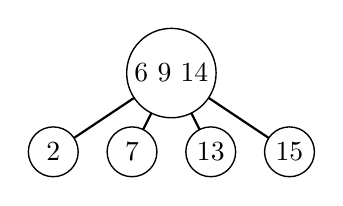
\begin{tikzpicture}
	\Vertex					{6 9 14}
	\Vertex[x=-1.5,y=-1]	{2}
	\Vertex[x=-0.5,y=-1]	{7}
	\Vertex[x=0.5,y=-1]		{13}
	\Vertex[x=1.5,y=-1]		{15}
	
	\Edge				(6 9 14)(2)
	\Edge				(6 9 14)(7)
	\Edge				(6 9 14)(13)
	\Edge				(6 9 14)(15)
\end{tikzpicture}
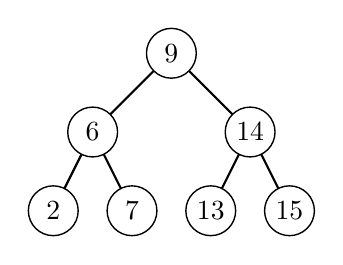
\begin{tikzpicture}
	\Vertex					{9}
	\Vertex[x=-1,y=-1]		{6}
	\Vertex[x=1,y=-1]		{14}
	\Vertex[x=-1.5,y=-2]	{2}
	\Vertex[x=-0.5,y=-2]	{7}
	\Vertex[x=0.5,y=-2]		{13}
	\Vertex[x=1.5,y=-2]		{15}
	
	\Edge			(9)(6)
	\Edge			(9)(14)
	\Edge			(6)(2)
	\Edge			(6)(7)
	\Edge			(14)(13)
	\Edge			(14)(15)
\end{tikzpicture}

			\caption{Step 7}
		\end{minipage}\hfill
		\begin{minipage}{.33\textwidth}
			\centering
			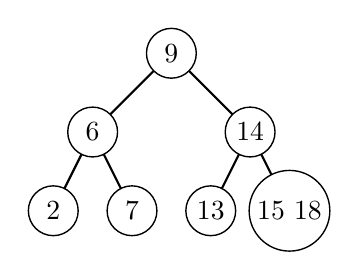
\begin{tikzpicture}
	\Vertex					{9}
	\Vertex[x=-1,y=-1]		{6}
	\Vertex[x=1,y=-1]		{14}
	\Vertex[x=-1.5,y=-2]	{2}
	\Vertex[x=-0.5,y=-2]	{7}
	\Vertex[x=0.5,y=-2]		{13}
	\Vertex[x=1.5,y=-2]		{15 18}
	
	\Edge			(9)(6)
	\Edge			(9)(14)
	\Edge			(6)(2)
	\Edge			(6)(7)
	\Edge			(14)(13)
	\Edge			(14)(15 18)
\end{tikzpicture}

			\caption{Step 8}
		\end{minipage}\hfill
		\begin{minipage}{.33\textwidth}
			\centering
			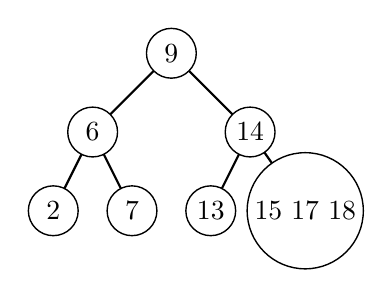
\begin{tikzpicture}
	\Vertex					{9}
	\Vertex[x=-1,y=-1]		{6}
	\Vertex[x=1,y=-1]		{14}
	\Vertex[x=-1.5,y=-2]	{2}
	\Vertex[x=-0.5,y=-2]	{7}
	\Vertex[x=0.5,y=-2]		{13}
	\Vertex[x=1.7,y=-2]		{15 17 18}
	
	\Edge			(9)(6)
	\Edge			(9)(14)
	\Edge			(6)(2)
	\Edge			(6)(7)
	\Edge			(14)(13)
	\Edge			(14)(15 17 18)
\end{tikzpicture}
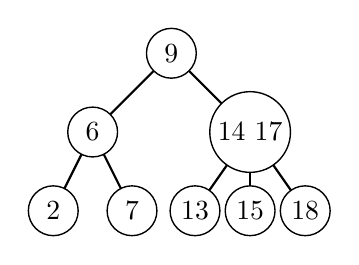
\begin{tikzpicture}
	\Vertex					{9}
	\Vertex[x=-1,y=-1]		{6}
	\Vertex[x=1,y=-1]		{14 17}
	\Vertex[x=-1.5,y=-2]	{2}
	\Vertex[x=-0.5,y=-2]	{7}
	\Vertex[x=0.3,y=-2]		{13}
	\Vertex[x=1,y=-2]		{15}
	\Vertex[x=1.7,y=-2]		{18}
	
	\Edge			(9)(6)
	\Edge			(9)(14 17)
	\Edge			(6)(2)
	\Edge			(6)(7)
	\Edge			(14 17)(13)
	\Edge			(14 17)(15)
	\Edge			(14 17)(18)
\end{tikzpicture}

			\caption{Step 9}
		\end{minipage}\hfill
	\end{figure}
\section{Relaxed AVL trees}
	First, we define $N(h)$ as a recurrence relation and prove its validity.\\
	Claim: \[N(h) =
				\begin{cases}
					1 & h=0\\
					2 & h=1\\
					3 & h=2\\
					N(h-1)+N(h-3)+1 & h > 2
				\end{cases}
			\]
	Proof: (Induction)\\
	$N(h)$ is defined as the minimum number of vertices in a Relaxed AVL tree. It is clear to see
	from this definition that the the three base cases hold.\\
	Suppose the claim holds for all $l<h$.\\
	We will now show that the claim also holds for $h$ by constructing the Relaxed AVL tree of height $h$ with the minimum number of vertices.
	Take one vertex and let it be the root of our new tree. Our tree must have height $h$, so at least one of its children must have height $h-1$.
	By our hypothesis, $N(h-1)$ is the minimum number of vertices in a Relaxed AVL tree of height $h-1$. In order to satisfy the Relaxed height-balance
	property, our tree's children's heights must not differ by more than two, so to minimize our vertices we shall choose our next child to have height $n-3$.
	Again, by our hypothesis we know that the minimum number of vertices in a Relaxed AVL tree of height $h-3$ is $N(h-3)$. If we now consider our tree
	with one root vertex and two children, both of which are also Relaxed AVL trees with $N(h-1)$ and $N(h-2)$ vertices, our number of vertices will be
	$N(h-1)+N(h-3)+1$. Thus our definition of $N(h)$ holds for all $h$.
	\newline
	\newline
	We will now show that $N(h)\in{\Omega{(k^h)}}$ for some $k>1$.\\
	It is sufficient to show that $N(h)\ge{ck^h}$ for some $c>0,k>1$.
	Claim: There exists some $c>0,k>1$ such that $N(h)\ge{ck^h}$ for all $h$.\\
	Proof: (Induction)
	\begin{align*}
		N(0)=1: \quad& 1\ge{ck^0}\quad\text{if}\quad\frac{1}{k^0}\ge{c}\\[1em]
		N(1)=2: \quad& 2\ge{ck^1}\quad\text{if}\quad\frac{1}{k^1}\ge{c}\\[1em]
		N(2)=3: \quad& 3\ge{ck^2}\quad\text{if}\quad\frac{1}{k^2}\ge{c}
	\end{align*}
	Note that the cases for $h=0$ and $h=1$ also hold when $c\le\frac{1}{k^2}$, so let $c\le\frac{1}{k^2}$.\\
	Suppose $N(l)\ge{ck^l}$ for all $l<h$.\\
	We want to show that $N(h)\ge{ck^h}$ for some $c>0,k>1$. Recall the definition for $N(h)$:
	\[N(h)=N(h-1)+N(h-3)+1\]
	By our hypothesis, we have
	\begin{align*}
		N(h)&\ge{ck^{h-1}+ck^{h-3}+1}\\
		&\ge{ck^{h-1}+ck^{h-3}}
	\end{align*}
	So if we can show that $ck^{h-1}+ck^{h-3}\ge{ck^h}$, it would be sufficient to show that $N(h)\ge{ck^h}$.
	\begin{align*}
		&ck^{h-1}+ck^{h-3}\ge{ck^h}\\
		&\implies{\frac{ck^{h-1}+ck^{h-3}}{ck^{h-3}}\ge{\frac{ck^h}{ck^{h-3}}}}\\
		&\implies{k^2+1\ge{k^3}}\\
		&\implies{k^3-k^2-1\le{0}}
	\end{align*}
	The real root of the polynomial $k^3-k^2-1=0$ is approximately $1.4655$, so any value for $k$ less than this
	value will do. Recall that we defined $c\le\frac{1}{k^2}$. So the claim holds for $k=1.4655$ and $c=\frac{1}{1.4655^2}$,
	and therefore $N(h)\ge{\frac{1}{1.4655^2}1.4655^{h}}$ for any value of $h$.\\
	Thus we have proven the claim that $N(h)\ge{ck^h}$ for some $c>0,k>1$, and therefore $N(h)\in\Omega{(1.4655^h)}$.

\end{document}
